\documentclass[12pt]{article}
\usepackage[french]{babel}
\usepackage[T1]{fontenc}
\usepackage{listings}
\usepackage{amsmath,amsthm,amssymb,amsfonts}
\usepackage[dvipsnames]{xcolor}
\usepackage{pgfpages}
\usepackage{fullpage}
\usepackage[unicode,psdextra]{hyperref}
\usepackage{graphics}
\usepackage{float}
\usepackage{fancyvrb}

\lstdefinestyle{codeblock}{
	keywordstyle=\color{magenta},
	basicstyle=\ttfamily\footnotesize,
	identifierstyle=\color{blue},
	numbersep=5pt,
	tabsize=2,
	breaklines=true,
	numbers=left,
	captionpos=b,
	frame=single
}
\lstset{style=codeblock}

\hypersetup{
	colorlinks,
	citecolor=black,
	filecolor=black,
	linkcolor=black,
	urlcolor=black
}

\title{Rapport de projet}

\begin{document}
\maketitle
\begin{figure}[H]
	\centering
	\begin{BVerbatim}
 _____  ______                               
|  __ \|  ____|                             
| |__) | |__ ___  _ __ _ __ ___   ___ _ __   
|  ___/|  __/ _ \| '__| '_ ` _ \ / _ | '__|
| |    | | | (_) | |  | | | | | |  __| |     
|_|    |_|  \___/|_|  |_| |_| |_|\___|_|   
	\end{BVerbatim}
\end{figure}
\tableofcontents
\newpage

\section{Introduction}

\begin{center}
	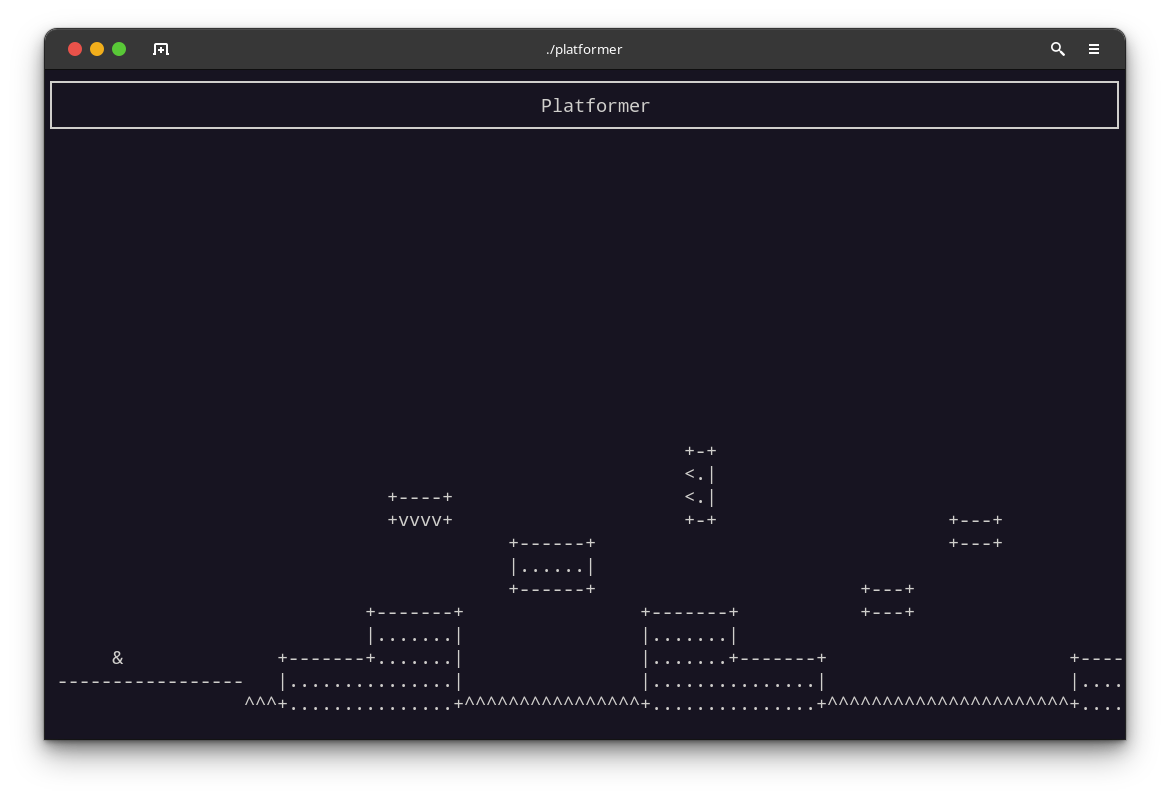
\includegraphics[width=0.90\textwidth]{content/image.png}
\end{center}

Platformer est un jeu de plateforme, où le but est d'arriver au bout d'une carte après de multiple obstacles. Ce jeu se rapproche de Mario Bros.

Le jeu est programmé en \textbf{C} et s'utilise dans une console (similaire a MS-DOS).

\section{Problèmes recontrés}

	\subsection{Chargement de la carte}
	
	\subsection{Physique et mouvement}
	
	\subsection{Affichage}
	
	\subsection{Collisions}
	
	
	\begin{lstlisting}[language=C, title={Programme en C}]
		int test;
	\end{lstlisting}

\section{Conclusion}

Parmi les idées qui auraient pû améliorer le jeu, nous avons retenu :
\begin{itemize}
	\item Un menu pour choisir la carte
	\item Des adversaires automatiques
	\item Des couleurs
	\item Éventuellement, un outil pour créer d'autres cartes (ou un guide)
	\item \dots
\end{itemize}
	
\end{document}